% CS615A Aspects of System Administration
% Author: Jan Schaumann <jschauma@netmeister.org>
% $Id: slides.tex,v 1.12 2006/02/27 02:53:29 jschauma Exp $
\special{! TeXDict begin /landplus90{true}store end }

\documentclass[xga]{xdvislides}
\usepackage[landscape]{geometry}
\usepackage{graphics}
\usepackage{graphicx}
\usepackage{colordvi}

\begin{document}
\setfontphv

%%% Headers and footers
\lhead{\slidetitle}                               % default:\lhead{\slidetitle}
\chead{CS615 - Aspects of System Administration}% default:\chead{\relax}
\rhead{Slide \thepage}                       % default:\rhead{\sectiontitle}
\lfoot{\Gray{Automating Administrative Tasks}}% default:\lfoot{\slideauthor}
\cfoot{\relax}                               % default:\cfoot{\relax}
\rfoot{\Gray{\today}}

\vspace*{\fill}
\begin{center}
	\Hugesize
		CS615 - Aspects of System Administration\\ [1em]
		Automating Administrative Tasks / Shell Scripting\\ [1em]

	\hspace*{5mm}\blueline\\ [1em]
	\Normalsize
		Department of Computer Science\\
		Stevens Institute of Technology\\
		Jan Schaumann\\
		\verb+jschauma@stevens.edu+\\
		\verb+http://www.cs.stevens.edu/~jschauma/615/+
\end{center}
\vspace*{\fill}

Systems Security Engineering Seminar Series
Verizon Data Breach Investigations Report
https://www.stevens.edu/news/content/systems-security-engineering-seminar-series-bhavesh-chauhan-security-solutions-verizon

%\subsection{Topics Covered}
%Overview:
%\begin{itemize}
%	\item why use automation
%	\item when to use automation
%	\item what tools to use
%\end{itemize}
%
%\subsection{Topics Covered}
%Overview:
%\begin{itemize}
%	\item why use automation
%	\item when to use automation
%	\item what tools to use
%\end{itemize}
%\addvspace{.5in}
%In more detail:
%\begin{itemize}
%	\item Shell Basics
%\end{itemize}
%
%\subsection{Topics Covered}
%Overview:
%\begin{itemize}
%	\item why use automation
%	\item when to use automation
%	\item what tools to use
%\end{itemize}
%\addvspace{.5in}
%In more detail:
%\begin{itemize}
%	\item Shell Basics
%	\item Regular Expressions
%\end{itemize}
%
%\subsection{Topics Covered}
%Overview:
%\begin{itemize}
%	\item why use automation
%	\item when to use automation
%	\item what tools to use
%\end{itemize}
%\addvspace{.5in}
%In more detail:
%\begin{itemize}
%	\item Shell Basics
%	\item Regular Expressions
%	\item Shell Programming
%\end{itemize}
%
%\subsection{Topics Covered}
%Overview:
%\begin{itemize}
%	\item why use automation
%	\item when to use automation
%	\item what tools to use
%\end{itemize}
%\addvspace{.5in}
%In more detail:
%\begin{itemize}
%	\item Shell Basics
%	\item Regular Expressions
%	\item Shell Programming
%	\item Perl, Python, ...
%\end{itemize}
%
%\subsection{Topics Covered}
%Overview:
%\begin{itemize}
%	\item why use automation
%	\item when to use automation
%	\item what tools to use
%\end{itemize}
%\addvspace{.5in}
%In more detail:
%\begin{itemize}
%	\item Shell Basics
%	\item Regular Expressions
%	\item Shell Programming
%	\item Perl, Python, ...
%	\item when only C will do
%\end{itemize}
%
%\subsection{Why?  When?  How?}
%Automating tasks has several benefits:
%\begin{itemize}
%	\item greater reliability
%\end{itemize}
%
%\subsection{Why?  When?  How?}
%Automating tasks has several benefits:
%\begin{itemize}
%	\item greater reliability
%	\item guaranteed regularity
%\end{itemize}
%
%\subsection{Why?  When?  How?}
%Automating tasks has several benefits:
%\begin{itemize}
%	\item greater reliability
%	\item guaranteed regularity
%	\item enhanced system efficiency
%\end{itemize}
%
%\subsection{Why?  When?  How?}
%Automating tasks has several benefits:
%\begin{itemize}
%	\item greater reliability
%	\item guaranteed regularity
%	\item enhanced system efficiency
%\end{itemize}
%\vspace{.5in}
%Automate tasks for
%\begin{itemize}
%	\item yourself
%\end{itemize}
%
\subsection{The 7 cardinal virtues of System Administrators}
\vspace*{\fill}
\begin{center}
	\includegraphics[scale=1.2]{pics/flexibility.eps}
\end{center}
\vspace*{\fill}

\subsection{The 7 cardinal virtues of System Administrators}
\vspace*{\fill}
\begin{center}
	
\includegraphics[scale=0.8]{pics/ingenuity.eps} \\
\end{center}
\vspace*{\fill}

%\subsection{The 7 cardinal virtues of System Administrators}
%\vspace*{\fill}
%\begin{center}
%	
\includegraphics[scale=0.55,angle=-90]{pics/ingenuity-can-should.eps}
%\end{center}
%\vspace*{\fill}
%
\subsection{The 7 cardinal virtues of System Administrators}
\vspace*{\fill}
\begin{center}
	
\includegraphics[scale=0.2]{pics/waldo.eps}
\end{center}
\vspace*{\fill}

\subsection{The 7 cardinal virtues of System Administrators}
\vspace*{\fill}
\begin{center}
	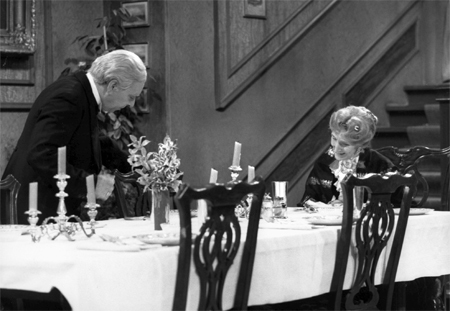
\includegraphics[scale=4]{pics/DinnerForOne.eps}
\end{center}
\vspace*{\fill}

\subsection{The 7 cardinal virtues of System Administrators}
\vspace*{\fill}
\begin{center}
	
\includegraphics[scale=0.8]{pics/try_try_again.eps}
\end{center}
\vspace*{\fill}

\subsection{The 7 cardinal virtues of System Administrators}
\vspace*{\fill}
\begin{center}
	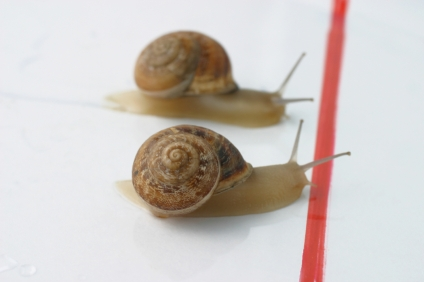
\includegraphics[scale=5]{pics/patience.eps}
\end{center}
\vspace*{\fill}

\subsection{The 7 cardinal virtues of System Administrators}
\vspace*{\fill}
\begin{center}
	
\includegraphics[scale=1.0]{pics/height_of_laziness.eps}
\end{center}
\vspace*{\fill}


\subsection{The 7 cardinal virtues of System Administrators}
\begin{itemize}
	\item flexibility
	\item ingenuity
	\item attention to detail
	\item adherence to routine
	\item persistence
	\item patience
	\item laziness
\end{itemize}

\subsection{The 7 cardinal virtues of System Administrators}
\begin{itemize}
	\item flexibility
	\item ingenuity
	\item attention to detail
	\item adherence to routine
	\item persistence
	\item patience
	\item laziness
\end{itemize}
\addvspace{.5in}

In addition:
\begin{itemize}
	\item impatience
	\item hubris
\end{itemize}

\subsection{Why?  When?  How?}
Automating tasks has several benefits:
\begin{itemize}
	\item greater reliability
	\item guaranteed regularity
	\item enhanced system efficiency
\end{itemize}
\vspace{.5in}
Automate tasks for
\begin{itemize}
	\item yourself
	\item other system administrators
\end{itemize}

\subsection{Why?  When?  How?}
Automating tasks has several benefits:
\begin{itemize}
	\item greater reliability
	\item guaranteed regularity
	\item enhanced system efficiency
\end{itemize}
\vspace{.5in}
Automate tasks for
\begin{itemize}
	\item yourself
	\item other system administrators
	\item all users
\end{itemize}


\subsection{Tools}
\vspace*{\fill}
\begin{center}
	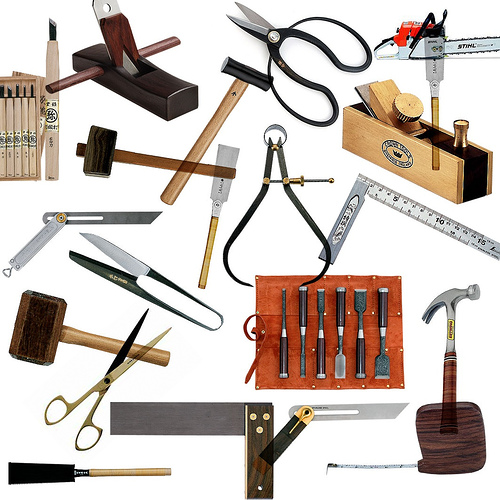
\includegraphics[scale=1.4]{pics/tools.eps}
\end{center}
\vspace*{\fill}

\subsection{The right tool?}
\vspace*{\fill}
\begin{center}
	
\includegraphics[scale=0.6]{pics/hammer.eps}
\end{center}
\vspace*{\fill}

\subsection{The right tool?}
\vspace*{\fill}
\begin{center}
	
\includegraphics[scale=2.5]{pics/nails.eps}
\end{center}
\vspace*{\fill}

\subsection{The right tool?}
\vspace*{\fill}
\begin{center}
	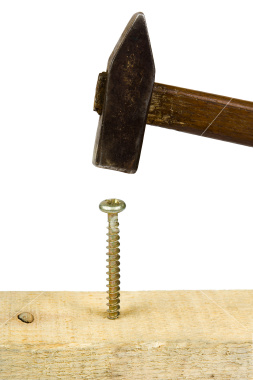
\includegraphics[scale=3]{pics/hammer-screw.eps}
\end{center}
\vspace*{\fill}

\subsection{A better hammer!}
\vspace*{\fill}
\begin{center}
	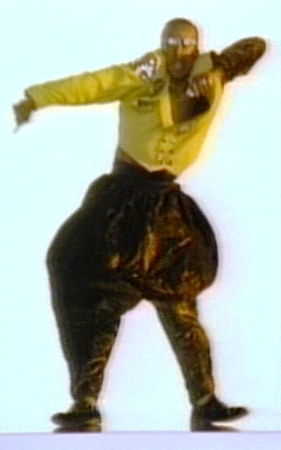
\includegraphics[scale=3]{pics/mchammer.eps}
\end{center}
\vspace*{\fill}


\subsection{Approaching Automation}
Three basic categories:
\\

\begin{itemize}
	\item scripting
	\item programming
	\item software development
\end{itemize}

\subsection{Approaching Automation}
Three basic categories:
\\
\begin{itemize}
	\item scripting
\end{itemize}
\vspace*{\fill}
\begin{center}
	
\includegraphics[scale=0.5]{pics/hammer.eps}
\end{center}
\vspace*{\fill}


\subsection{Approaching Automation}
Three basic categories:
\\

\begin{itemize}
	\item scripting
		\begin{itemize}
			\item automating {\em very} simple tasks
		\end{itemize}
\end{itemize}

\subsection{Approaching Automation}
Three basic categories:
\\

\begin{itemize}
	\item scripting
		\begin{itemize}
			\item automating {\em very} simple tasks
			\item customization of user environment
		\end{itemize}
\end{itemize}

\subsection{Approaching Automation}
Three basic categories:
\\

\begin{itemize}
	\item scripting
		\begin{itemize}
			\item automating {\em very} simple tasks
			\item customization of user environment
			\item often only suitable for one individual user
		\end{itemize}
\end{itemize}

\subsection{Approaching Automation}
Three basic categories:
\\

\begin{itemize}
	\item scripting
		\begin{itemize}
			\item automating {\em very} simple tasks
			\item customization of user environment
			\item often only suitable for one individual user
			\item usually eventually evolves into larger programs
		\end{itemize}
\end{itemize}


\subsection{Approaching Automation}
Three basic categories:
\\

\begin{itemize}
	\item programming
\end{itemize}
\vspace*{\fill}
\begin{center}
	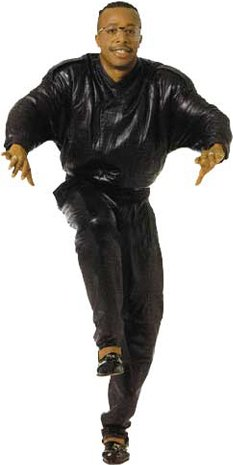
\includegraphics[scale=0.6]{pics/mchammer2.eps}
\end{center}
\vspace*{\fill}

\subsection{Approaching Automation}
Three basic categories:
\\

\begin{itemize}
	\item programming
\end{itemize}
\vspace*{\fill}
\begin{center}
	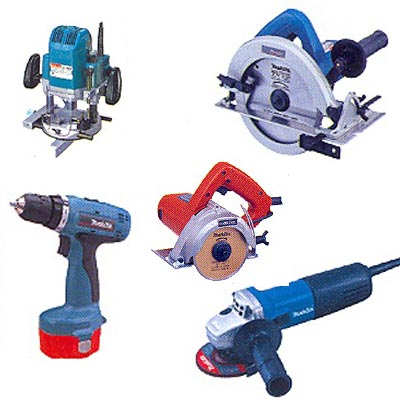
\includegraphics[scale=0.8]{pics/power-tools.eps}
\end{center}
\vspace*{\fill}



\subsection{Approaching Automation}
Three basic categories:
\\

\begin{itemize}
	\item programming
		\begin{itemize}
			\item suitable for simple to moderately complex tasks
		\end{itemize}
\end{itemize}

\subsection{Approaching Automation}
Three basic categories:
\\

\begin{itemize}
	\item programming
		\begin{itemize}
			\item suitable for simple to moderately complex tasks
			\item results frequently used by a small base of users
		\end{itemize}
\end{itemize}

\subsection{Approaching Automation}
Three basic categories:
\\

\begin{itemize}
	\item programming
		\begin{itemize}
			\item suitable for simple to moderately complex tasks
			\item results frequently used by a small base of users
			\item uses basic framework or common toolkits
		\end{itemize}
\end{itemize}

\subsection{Approaching Automation}
Three basic categories:
\\

\begin{itemize}
	\item programming
		\begin{itemize}
			\item suitable for simple to moderately complex tasks
			\item results frequently used by a small base of users
			\item uses basic framework or common toolkits
			\item provides consistent interface
		\end{itemize}
\end{itemize}

\subsection{Approaching Automation}
Three basic categories:
\\

\begin{itemize}
	\item programming
		\begin{itemize}
			\item suitable for simple to moderately complex tasks
			\item results frequently used by a small base of users
			\item uses basic framework or common toolkits
			\item provides consistent interface
			\item may evolve into full product
		\end{itemize}
\end{itemize}

\subsection{Approaching Automation}
Three basic categories:
\\

\begin{itemize}
	\item software development
\end{itemize}
\vspace*{\fill}
\begin{center}
	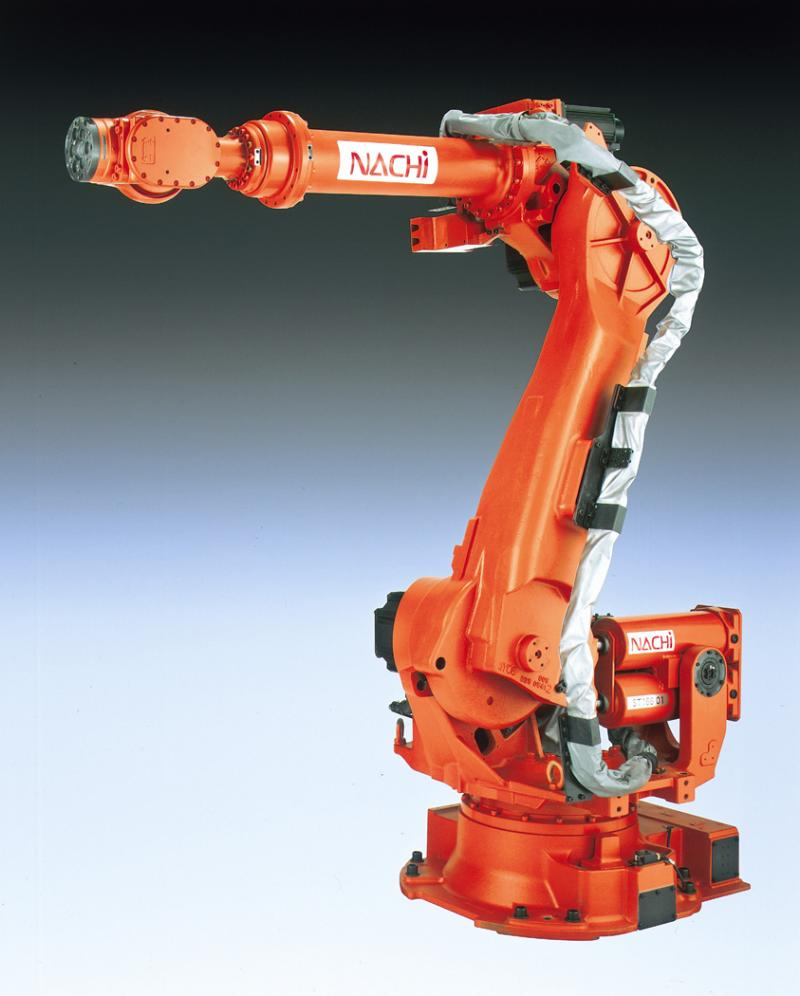
\includegraphics[scale=0.25]{pics/big-tool.eps}
\end{center}
\vspace*{\fill}


\subsection{Approaching Automation}
Three basic categories:
\\

\begin{itemize}
	\item software development
		\begin{itemize}
			\item required for any reasonably complex task
		\end{itemize}
\end{itemize}

\subsection{Approaching Automation}
Three basic categories:
\\

\begin{itemize}
	\item software development
		\begin{itemize}
			\item required for any reasonably complex task
			\item uses formal software engineering approach (measurable goals,
				requirements, specifications, ...)
		\end{itemize}
\end{itemize}

\subsection{Approaching Automation}
Three basic categories:
\\

\begin{itemize}
	\item software development
		\begin{itemize}
			\item required for any reasonably complex task
			\item uses formal software engineering approach (measurable goals,
				requirements, specifications, ...)
			\item may evolve from previous prototypes
		\end{itemize}
\end{itemize}


\subsection{Approaching Automation}
Three basic categories:
\\

\begin{itemize}
	\item software development
		\begin{itemize}
			\item required for any reasonably complex task
			\item uses formal software engineering approach (measurable goals,
				requirements, specifications, ...)
			\item may evolve from previous prototypes
			\item requires ongoing continous maintenance / development efforts
		\end{itemize}
\end{itemize}


\newpage
\vspace*{\fill}
\begin{center}
	\Hugesize
		Jan's Words of Wisdom \\ [1em]
	\hspace*{5mm}
	\blueline\\
	\hspace*{5mm}\\
		Tuesday, February 19th, 2013
\end{center}
\vspace*{\fill}

\subsection{Words of Wisdom}
\\

\newcommand{\gargantuan}{\fontsize{60}{65}\selectfont}
\gargantuan
\begin{center}
Anything you do more than once is worth automating.
\end{center}
\Normalsize

\subsection{Words of Wisdom}
\vspace*{\fill}
\begin{center}
	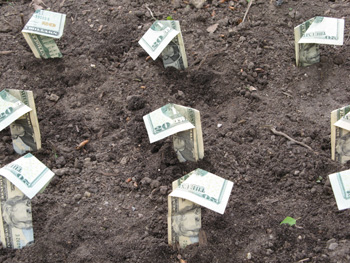
\includegraphics[scale=3.0]{pics/growmoney.eps}
\end{center}
\vspace*{\fill}

\subsection{Words of Wisdom}
\vspace*{\fill}
\begin{center}
	
\includegraphics[scale=3.5]{pics/money-tree.eps}
\end{center}
\vspace*{\fill}

\subsection{Good tools exhibit our cardinal virtues}
Our software defines, exhibits or provides:
\begin{itemize}
	\item flexibility
	\item ingenuity
	\item attention to detail
	\item adherence to routine
	\item persistence
	\item patience
	\item laziness
\end{itemize}

\subsection{Things to automate}
\begin{itemize}
	\item software installation and upgrades
	\item user account creation and deletion
	\item system configuration
	\item log and event processing
	\item {\em pretty much everything, seriously}
\end{itemize}

%\subsection{Scheduling programs}
%
%\begin{itemize}
%	\item repeatedly $\rightarrow$ \verb+cron(8)+, \verb+crontab(1)+ \\
%		\verb,30 5 * * 6 find /tmp -type f -mtime +7 -atime +7 -exec rm -f '{}' ';',
%	\item once $\rightarrow$ \verb+at(1)+ \\
%		\verb,at -f script.sh 1am tomorrow,
%	\item based on system load $\rightarrow$ \verb+batch(1)+ \\
%		\verb,batch -f script.sh 4pm + 3 days,
%\end{itemize}
%

\newpage
\vspace*{\fill}
\begin{center}
    \Hugesize
        It's coding time! \\ [1em]
    \hspace*{5mm}
    \blueline\\
    \hspace*{5mm}\\
	Get out your laptops...
\end{center}
\vspace*{\fill}

\subsection{Shell Essentials}
Essential Tools:
\begin{itemize}
	\item pipes
	\item ls(1), find(1)
	\item grep(1)
	\item awk(1)
	\item sed(1)
	\item tr(1)
	\item sort(1)
	\item regular expressions
	\item ssh(1)/scp(1)
	\item wc(1)
	\item expect(1)
\end{itemize}

\subsection{Coding time!}
Page view statistics for Wikimedia projects \\
{\tt http://dumps.wikimedia.org/other/pagecounts-raw/} \\
\vspace{.5in}

On {\tt linux-lab.cs.stevens.edu}:
\begin{verbatim}
ls ~jschauma/public_html/615/pagecounts-20130201-000000.gz
\end{verbatim}

\subsection{Coding time!}
\begin{itemize}
	\item How many unique objects were requested in that hour in total?
	\item For {\tt en} only:
		\begin{itemize}
			\item How many unique objects were requested?
			\item Which is the most often requested object?
			\item How many requests in total?
			\item How much data was transferred in total?
			\item Which was the largest object requested?
			\item What is the longest word found on the ten most
				frequently retrieved pages?
		\end{itemize}
\end{itemize}

\subsection{Coding time!}
How many unique objects were requested?

\begin{verbatim}
FILE=~jschauma/public_html/615/pagecounts-20130201-000000.gz
zcat ${FILE} | wc -l
\end{verbatim}

\subsection{Coding time!}
How many unique objects were requested for {\tt en} only?

\begin{verbatim}
FILE=~jschauma/public_html/615/pc
grep "^en " ${FILE} | wc -l
\end{verbatim}

\subsection{Coding time!}
Which is the most often requested object?

\begin{verbatim}
FILE=~jschauma/public_html/615/pc
grep "^en " ${FILE} | sort -k3 -n | tail -1
\end{verbatim}

\subsection{Coding time!}
How many requests were there in total?

\begin{verbatim}
awk '{ sum=sum+$(NF-1); }; END { print sum; }' en
\end{verbatim}

\subsection{Coding time!}
How much data was transferred in total?

\begin{verbatim}
echo $(( $(awk '{ sum=sum+$NF; }; END { print sum; }' en)/1024/1024/1024 ))
\end{verbatim}

\subsection{Coding time!}
Which was the largest object requested?

\begin{verbatim}
FILE=en
awk '{ s=$NF/$(NF-1); if (s>l) { l=s; n=$0; }}; END { print n; }' <en
\end{verbatim}

\subsection{Coding time!}
What is the longest word found on the ten most frequently retrieved pages?

\begin{verbatim}
for f in $(cat en | sort -k3 -n | tail -10 |
        sed -e 's/en \(.*\) [0-9]* [0-9]*/\1/'); do
        links -dump http://en.wikipedia.org/wiki/${f}
done |
tr '[:punct:]' ' ' |
tr '[:space:]' '\n' |
tr '[:upper:]' '[:lower:]' |
egrep '^[a-z]+$' |
awk '{ print length() " " $0; }' |
sort -n |
tail -1
\end{verbatim}

\subsection{Writing Shell Scripts}
{\tt sh examples/shexamples}

\subsection{Writing Shell Scripts: Builtins, Functions, Job Control, Signals}
\begin{itemize}
	\item {\em builtins} are executed internally (ie without spawning a
		new process)
\end{itemize}

\subsection{Writing Shell Scripts: Builtins, Functions, Job Control, Signals}
\begin{itemize}
	\item {\em builtins} are executed internally (ie without spawning a
		new process)
	\item some {\em builtins} cannot be performed (efficiently) by
		separate processes, some can (and are)
\end{itemize}

\subsection{Writing Shell Scripts: Builtins, Functions, Job Control, Signals}
\begin{itemize}
	\item {\em builtins} are executed internally (ie without spawning a
		new process)
	\item some {\em builtins} cannot be performed (efficiently) by
		separate processes, some can (and are)
	\item {\em functions} are executed within the current shell
\end{itemize}

\subsection{Writing Shell Scripts: Builtins, Functions, Job Control, Signals}
\begin{itemize}
	\item {\em builtins} are executed internally (ie without spawning a
		new process)
	\item some {\em builtins} cannot be performed (efficiently) by
		separate processes, some can (and are)
	\item {\em functions} are executed within the current shell
	\item job control may work differently within {\em functions}
\end{itemize}

\subsection{Writing Shell Scripts: Builtins, Functions, Job Control, Signals}
\begin{itemize}
	\item {\em builtins} are executed internally (ie without spawning a
		new process)
	\item some {\em builtins} cannot be performed (efficiently) by
		separate processes, some can (and are)
	\item {\em functions} are executed within the current shell
	\item job control may work differently within {\em functions}
	\item {\em functions} operate on and influence the current environment
\end{itemize}

\subsection{Writing Shell Scripts: Builtins, Functions, Job Control, Signals}
\begin{itemize}
	\item {\em builtins} are executed internally (ie without spawning a
		new process)
	\item some {\em builtins} cannot be performed (efficiently) by
		separate processes, some can (and are)
	\item {\em functions} are executed within the current shell
	\item job control may work differently within {\em functions}
	\item {\em functions} operate on and influence the current environment
	\item shells can monitor and control {\em jobs}
\end{itemize}

\subsection{Writing Shell Scripts: Builtins, Functions, Job Control, Signals}
\begin{itemize}
	\item {\em builtins} are executed internally (ie without spawning a
		new process)
	\item some {\em builtins} cannot be performed (efficiently) by
		separate processes, some can (and are)
	\item {\em functions} are executed within the current shell
	\item job control may work differently within {\em functions}
	\item {\em functions} operate on and influence the current environment
	\item shells can monitor and control {\em jobs}
	\item some {\em signals} may be ignored or caught and handled, others
		may not be ignored
\end{itemize}

\subsection{Writing Shell Scripts: Builtins, Functions, Job Control, Signals}
\begin{itemize}
	\item {\em builtins} are executed internally (ie without spawning a
		new process)
	\item some {\em builtins} cannot be performed (efficiently) by
		separate processes, some can (and are)
	\item {\em functions} are executed within the current shell
	\item job control may work differently within {\em functions}
	\item {\em functions} operate on and influence the current environment
	\item shells can monitor and control {\em jobs}
	\item some {\em signals} may be ignored or caught and handled, others
		may not be ignored
\end{itemize}
\addvspace{.5in}
As you can tell, this whole thing looks like a full-blown programming language!

%
%\subsection{Regular Expressions}
%A regular expression is a pattern that describes a set of strings. \\
%
%\begin{itemize}
%	\item patterns can be
%		\begin{itemize}
%			\item single characters (\verb+a+)
%			\item a bracket expression, such as
%				\begin{itemize}
%					\item a number of characters -- \verb+[aK2l,]+
%					\item a range expression -- \verb+[a-z]+
%					\item a negated bracket expression -- \verb+[^0-9]+
%				\end{itemize}
%			\item a character with a special meaning, such as
%				\begin{itemize}
%					\item \verb+.+ -- any single character
%					\item \verb+^+ -- beginning of line
%					\item \verb+$+ -- end of line
%				\end{itemize}
%			\item a combination of patterns
%		\end{itemize}
%\end{itemize}
%
%\subsection{Regular Expressions}
%\begin{itemize}
%	\item patterns can be followed by qualifiers and quantifiers
%		\begin{itemize}
%			\item \verb+?+ -- the pattern is optional and matched at most once
%			\item \verb+*+ -- the pattern will be matched zero or more times
%			\item \verb|+| -- the pattern will be matched one or more times
%			\item \verb+{n}+ -- the pattern is matched exactly \verb+n+ times
%			\item \verb+{n,}+ -- the pattern is matched \verb+n+ or more times
%			\item \verb+{n,m}+ -- the pattern is matched at least \verb+n+,
%				but no more than \verb+m+ times
%		\end{itemize}
%	\item patterns can be logically grouped together \verb+(1[a-z]2|a[0-9]z)+
%	\item matched patterns can be remembered and referenced lateron
%\end{itemize}
%\addvspace{.5in}
%NB: different tools implement regular expressions somewhat differently
%
%\subsection{Regular Expressions}
%Example exercises:
%\begin{itemize}
%	\item extract all proper words from a document
%	\item extract all URLs from a document
%	\item check if a string is a valid IPv4 address
%	\item check if a string is a valid IPv6 address
%	\item check if a string is a valid date
%\end{itemize}
%
\newpage
\vspace*{\fill}
\begin{center}
    \Hugesize
        Hooray! \\ [1em]
    \hspace*{5mm}
    \blueline\\
    \hspace*{5mm}\\
        5 Minute Break
\end{center}
\vspace*{\fill}
%
%\subsection{Scripting / interpreted Languages}
%\vspace*{\fill}
%\begin{center}
%	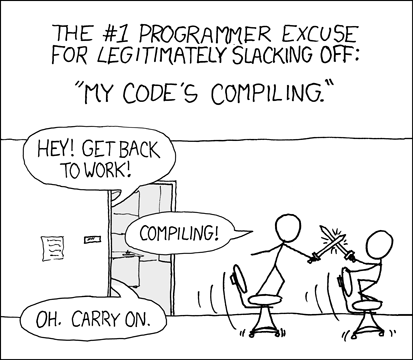
\includegraphics[scale=0.9]{pics/compiling.eps}
%	\\
%	\small \verb+http://xkcd.com/303/+
%\end{center}
%\vspace*{\fill}
%
%\subsection{Scripting / interpreted Languages}
%\\
%
%\Huge
%\begin{center}
%	Perl, Python, Ruby, \\
%	\addvspace{.5in}
%	PHP, Lisp, Smalltalk, Tcl, \\
%	\addvspace{.5in}
%	ECMA (JavaScript etc.), Lua
%\end{center}
%\Normalsize
%
%
%\subsection{Scripting / interpreted Languages}
%General advantages:
%\begin{itemize}
%	\item short development cycle
%	\item normally facilitates things like string manipulation,
%		arithmetic and more complex regular expressions
%	\item easily handles multiple file handles and other I/O
%	\item some security features
%	\item tens of thousands of special- and general-purpose modules
%		available
%\end{itemize}
%
%\subsection{Scripting / interpreted Languages}
%General disadvantages:
%\begin{itemize}
%	\item no one tool fits all purposes
%	\item tens of thousands of special- and general-purpose modules
%		available $\rightarrow$ lots of duplication, stale code,
%		questionable quality
%	\item security features frequently neglected or circumvented ("too
%		hard" or more precisely "inconvenient")
%	\item everybody has their particular favorite (and dislikes one or
%		the other)
%	\item interpreter not (necessarily) universally available /
%		installed
%\end{itemize}
%
%\subsection{When only C will do}
%\begin{itemize}
%	\item often faster / more efficient
%	\item inherent part of UNIX
%	\item scales better
%	\item enough rope to hang yourself
%	\item Face it:  you need to know C anyway
%\end{itemize}
%
%\subsection{User Interface}
%\\
%\vspace*{\fill}
%\begin{center}
%	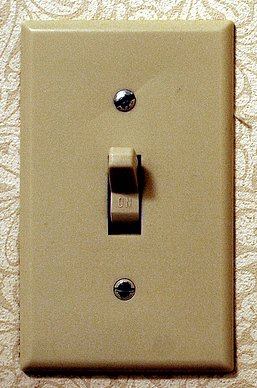
\includegraphics[scale=3]{pics/switch.eps}
%\end{center}
%\vspace*{\fill}
%
%\subsection{Unix Philosophy}
%\\
%\vspace*{\fill}
%\begin{center}
%	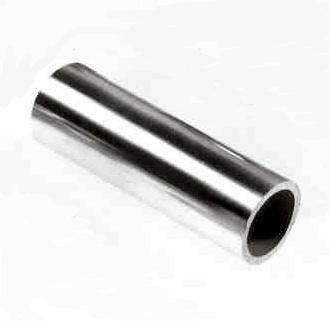
\includegraphics[scale=1.5]{pics/pipe.eps}
%\end{center}
%\vspace*{\fill}
%
%\subsection{Unix Philosophy}
%\\
%\Huge
%\begin{center}
%	Do one thing and do it well.
%\end{center}
%\Normalsize
%
%\subsection{The KISS Principle}
%\\
%\vspace*{\fill}
%\begin{center}
%	
\includegraphics[scale=0.3]{pics/kiss.eps}
%\end{center}
%\vspace*{\fill}
%
%\subsection{POLA}
%Principle of Least Astonishment
%\\
%\vspace*{\fill}
%\begin{center}
%	
\includegraphics[scale=0.8]{pics/kinder-surprise.eps}
%\end{center}
%\vspace*{\fill}
%
%\subsection{Test Driven}
%\vspace*{\fill}
%\begin{center}
%	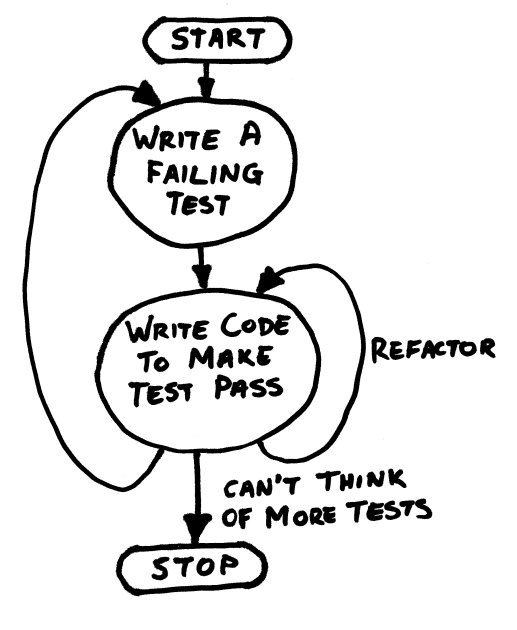
\includegraphics[scale=2.0]{pics/tdd.eps}
%\end{center}
%\vspace*{\fill}
%
%
%\subsection{The Zen of Python}
%\Huge
%\begin{center}
%Beautiful is better than ugly.
%\end{center}
%
%\subsection{The Zen of Python}
%\begin{center}
%Explicit is better than implicit.
%\end{center}
%
%\subsection{The Zen of Python}
%\begin{center}
%    Simple is better than complex.
%\vspace*{\fill}
%	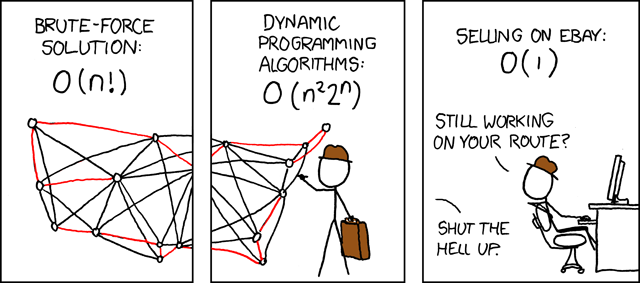
\includegraphics[scale=0.8]{pics/complexity.eps}
%	\\
%	\small \verb+http://xkcd.com/399/+
%\end{center}
%\vspace*{\fill}
%\Huge
%
%\subsection{The Zen of Python}
%\begin{center}
%    Complex is better than complicated.
%\end{center}
%
%\subsection{The Zen of Python}
%\begin{center}
%    Flat is better than nested.
%\end{center}
%
%\subsection{The Zen of Python}
%\begin{center}
%    Sparse is better than dense.
%\end{center}
%
%\subsection{The Zen of Python}
%\begin{center}
%    Readability counts.
%\end{center}
%
%\subsection{The Zen of Python}
%\begin{center}
%    Special cases aren't special enough to break the rules.
%\end{center}
%
%\subsection{The Zen of Python}
%\begin{center}
%    Special cases aren't special enough to break the rules. \\
%\addvspace{.5in}
%    Although practicality beats purity.
%\end{center}
%
%\subsection{The Zen of Python}
%\\
%\begin{center}
%    Errors should never pass silently.
%\end{center}
%
%\subsection{The Zen of Python}
%\\
%\begin{center}
%    Errors should never pass silently. \\
%\addvspace{.2in}
%	\small
%	(That would be implicitly accepted failure.)
%\end{center}
%\Huge
%
%\subsection{The Zen of Python}
%\\
%\begin{center}
%    Errors should never pass silently. \\
%\addvspace{.2in}
%	\small
%	(That would be implicitly accepted failure.) \\
%\addvspace{.2in}
%	(You know what would be better than something {\em implicit}?)
%\end{center}
%
%\subsection{The Zen of Python}
%\\
%\begin{center}
%    Errors should never pass silently. \\
%\addvspace{.2in}
%	\small
%	(That would be implicitly accepted failure.) \\
%\addvspace{.2in}
%	(You know what would be better than something {\em implicit}?) \\
%\addvspace{.2in}
%	(Why, of course, something {\em explicit}!)
%\end{center}
%
%\subsection{The Zen of Python}
%\\
%\begin{center}
%    Errors should never pass silently. \\
%\addvspace{.5in}
%    Unless explicitly silenced.
%\end{center}
%
%\subsection{The Zen of Python}
%\begin{center}
%    In the face of ambiguity, refuse the temptation to guess.
%\end{center}
%
%\subsection{The Zen of Python}
%\begin{center}
%    There should be one -- and preferably only one -- obvious way to do it.
%\end{center}
%
%\subsection{The Zen of Python}
%\begin{center}
%    There should be one -- and preferably only one -- obvious way to do it.
%
%\addvspace{.5in}
%
%    Although that way may not be obvious at first unless you're Dutch. \\
%\vspace*{\fill}
%	
\includegraphics[scale=0.5]{pics/sign.eps}
%\end{center}
%
%
%\subsection{The Zen of Python}
%\begin{center}
%    Now is better than never.
%\end{center}
%
%\subsection{The Zen of Python}
%\begin{center}
%    Now is better than never.  \\
%
%\addvspace{.5in}
%
%    Although never is often better than *right* now.
%\end{center}
%
%\subsection{The Zen of Python}
%\begin{center}
%    If the implementation is hard to explain, it's a bad idea.
%\end{center}
%
%\subsection{The Zen of Python}
%\begin{center}
%    If the implementation is easy to explain, \\
%	it {\em may} be a good idea.
%\end{center}
%
%\subsection{A simple interface, easy to explain.  Yet...}
%\\
%\vspace*{\fill}
%\begin{center}
%	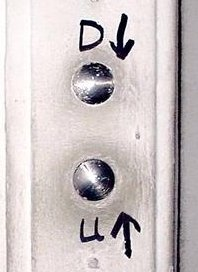
\includegraphics[scale=1.2]{pics/elevator_buttons-reverse.eps}
%\end{center}
%\vspace*{\fill}
%
%
%\subsection{The Zen of Python}
%\begin{center}
%    Namespaces are one honking great idea -- let's do more of those!
%\end{center}
%\Normalsize
%
%\subsection{Documentation}
%\vspace*{\fill}
%\begin{center}
%	\includegraphics[scale=0.9]{pics/manual.eps}
%	\hspace{.5in}
%	\includegraphics[scale=0.9]{pics/manual2.eps}
%	\\
%	\vspace{.2in}
%	\Huge
%	{\bf WTFM}
%	\Normalsize
%\end{center}
%\vspace*{\fill}
%
%
%\subsection{Consistency}
%\vspace*{\fill}
%\begin{center}
%	
\includegraphics[scale=1.1]{pics/consistency.eps}
%\end{center}
%\vspace*{\fill}
%
%\subsection{Robustness Principle or Postel's Law}
%\\
%\Huge
%\begin{center}
%	Be conservative in what you do; be liberal in what you accept from others.
%\end{center}
%\Normalsize
%
%\subsection{Avoid the Quick Fix}
%\\
%\Huge
%\begin{center}
%	There's nothing as permanent as a temporary solution.
%\end{center}
%\Normalsize
%
%\subsection{Take a good look in the mirror!}
%\\
%\vspace*{\fill}
%\begin{center}
%	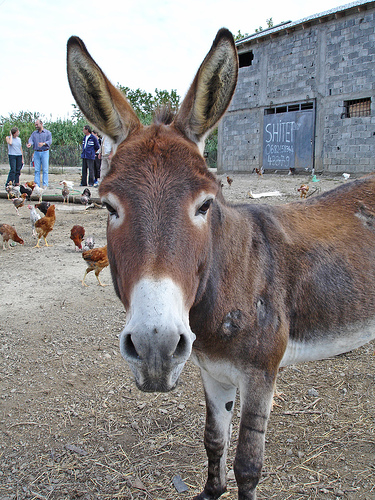
\includegraphics[scale=0.65]{pics/donkey.eps} \\
%	\small
%	Nice Ass!
%\end{center}
%\vspace*{\fill}
%
%\subsection{Take a good look in the mirror!}
%\\
%\Huge
%\begin{center}
%	Until you can {\em prove} otherwise, \\
%	assume that {\em you} are the Ass!
%\end{center}
%\Normalsize
%
%\subsection{Avoid the Project That Was Never Finished}
%\\
%\Huge
%\begin{center}
%	Don't let the Perfect be the enemy of the Good.
%\end{center}
%\Normalsize
%
%\subsection{Avoid Feature Creep}
%\vspace*{\fill}
%\begin{center}
%	
\includegraphics[scale=1.0]{pics/feeping.eps} \\
%	\small
%	\verb+http://www.feepingcreatures.com+
%\end{center}
%\vspace*{\fill}
%
%\subsection{Release Early, Release Often}
%\\
%\Huge
%\begin{center}
%	``More users find more bugs.'' \\
%	\addvspace{.2in}
%	\small F. Brooks, ``The Mythical Man Month''
%\end{center}
%\Normalsize
%
%\subsection{Increase the Bus Factor}
%\vspace*{\fill}
%\begin{center}
%	\includegraphics[scale=0.85]{pics/bert-ernie.eps} \\
%	\small
%	``Just friends.''
%\end{center}
%\vspace*{\fill}
%
%\subsection{Fix Broken Windows}
%\vspace*{\fill}
%\begin{center}
%	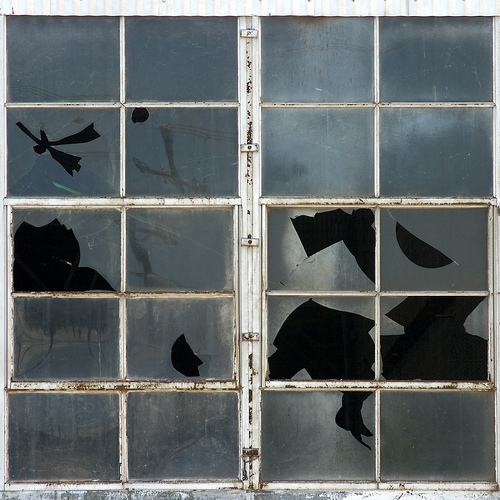
\includegraphics[scale=0.7]{pics/broken-windows.eps}
%\end{center}
%\vspace*{\fill}
%
%\subsection{Program Maintenance}
%\\
%\Huge
%\begin{center}
%	``... is an entropy-increasing process, and even its most skillful
%	execution only delays the subsidence of the system into unfixable
%	obsolescence.'' \\
%	\addvspace{.2in}
%	\small F. Brooks, ``The Mythical Man Month''
%\end{center}
%\Normalsize
%
%\subsection{Toss it!}
%\vspace*{\fill}
%\begin{center}
%	
\includegraphics[scale=3]{pics/waste.eps}
%\end{center}
%\vspace*{\fill}
%
%\subsection{Starting fresh}
%\vspace*{\fill}
%\begin{center}
%	
\includegraphics[scale=2]{pics/clean-slate.eps}
%\end{center}
%\vspace*{\fill}
%
%
\subsection{Reading}
Shell:
\begin{itemize}
	\item \verb+http://www.tldp.org/HOWTO/Bash-Prog-Intro-HOWTO.html+
	\item \verb+http://www.tldp.org/LDP/abs/html/+
	\item \verb+http://sed.sourceforge.net/sed1line.txt+
	\item \verb+csh(1)+, \verb+ksh(1)+, \verb+sh(1)+
	\item {\em Frisch}: Chapter 3, 14
\end{itemize}
%Perl:
%\begin{itemize}
%	\item \verb+http://www.perl.com+
%	\item \verb+http://www.cpan.org+
%	\item \verb+perl(1)+, \verb+perldoc(1)+, \verb+perlfaq(1)+
%\end{itemize}
%Python:
%\begin{itemize}
%	\item \verb+http://www.python.org+
%	\item \verb+http://www.samag.com/documents/s=8964/sam0312a/0312a.htm+
%	\item pydoc
%\end{itemize}

\end{document}
